\section[What is Cloud Computing?]{\textbf{What is Cloud Computing?} \\ \textit{Điện toán đám mây là gì}}



\subsection[What is a server composed of?]{\textbf{What is a server composed of?} \\
\textit{Máy chủ gồm những thành phần nào} }

\begin{itemize}
	\item Compute (tính toán): CPU
	\item Memory (bộ nhớ): RAM
	\item Storage (kho lưu trữ): Data
	\item Database (Cơ sở dữ liệu): Store data in a structured way (Lưu trữ dữ liệu một cách có cấu trúc)
	\item Network (mạng lưới): Routers (bộ định tuyến), switch (bộ chuyển mạch), DNS server (Máy chủ DNS)
\end{itemize}
\subsection[IT Terminology]{\textbf{IT Terminology} \\ \textit{Thuật ngữ IT}}

\begin{itemize}
	\item Network (mạng lưới): bao gồm các loại dây cáp (cables), các bộ định tuyến (routers) và các máy chủ được kết nối với nhau.
	\item Router (bộ định tuyến): Một mạng lưới các thiết bị dùng chuyển tiếp các gói dữ liệu giữa các mạng lưới máy tính. Nó biết nơi cần gửi các gói dữ liệu của bạn trên internet.
	\item Switch (bộ chuyển đổi): Nhận gói dữ liệu và gửi nó đến chính xác máy chủ/ người dùng trên network của bạn 
\end{itemize}

\subsection [Problems with traditional IT approach]{\textbf{Problems with traditional IT approach} \\ \textit{Các vấn đề với cách tiếp cận CNTT truyền thống}}

\begin{itemize}
	\item Pay for the rent the data center (Trả tiền thuê cho trung tâm dữ liệu)
	\item Pay for power supply, cooling, maintenance (Trả tiền cho nguồn điện, hệ thống làm mát và bảo trì, bảo dưỡng)
	\item Adding and replacing hardware takes time (Việc thêm và thay thế thiết bị phần cứng tốn thời gian)
	\item Scaling is limited (Việc mở rộng bị giới hạn)
	\item Hire 24/7 team to monitor the infrastructure (Thuê đổi ngũ trực 24/7 để giám sát hạ tầng)
	\item How to deal with disasters? (earthquake, power shutdown, fire, ...) (Làm sao để ứng phó với các sự cố ? (động đất, mất điện, cháy, ...))
	
\end{itemize}

\subsection[What is Cloud Computing?]{\textbf{What is Cloud Computing?} \\
	 \textit{Điện toán đám mây là gì?} }
\begin{itemize}
	\item Cloud computing is the on-demand delivery of compute power, database storage, applications, and other IT resources (Điện toán đám mây là hình thức cung cấp theo yêu cầu sức mạng tính toán, lưu trữ cơ sở dữ liệu, ứng, và các tài nguyên công nghệ thông tin khác)
	\item Through a cloud services platform with pay-as-you-go pricing (Thông qua một nền tảng dịch vụ đám mây với mô hình tính phí theo mức sử dụng)
	\item You can provision exactly the right type and size of computing resources you need (Bạn có thể triển khai một cách chính xác đúng với kiểu và kích thước tính toán tài nguyên mà bạn cần)
	\item You can access as many resources as you need, almost instantly (Bạn có thể truy cập nhiều tài nguyên mà bạn cần, gần như ngay lập tức)
	\item Simple way to access servers, storage, databases and a set of application services (Một cách đơn giản để truy cập các máy chủ, kho lưu trữ, các cơ sở dữ liệu và một tập hợp dịch vụ ứng dụng)
	\item Amazon Web Service owns and maintains the network-connected hardware required for these application services, while you provision and use what you need via a web application (Amazon Web Service sở hữu và duy trì thiết bị phần cứng kết nối mạng lưới cần thiết cho các dịch vụ ứng dụng này trong khi bạn triển khai và sử dụng thông qua một ứng dụng web)
\end{itemize}

\subsection[You've been using some Could services]{\textbf{You've been using some Could services } \\ \textit{Bạn đang sử dụng vài dịch vụ đám mây}}
\begin{itemize}
	\item Gmail
	\begin{itemize}
		\item E-mail cloud service (Dịch vụ đám mấy E-mail)
		\item Pay for only your emails stored (no infrastructure, etc.) (Bạn chỉ phải trả tiền cho số email của bạn được lưu trữ (không phải trả chi phí cho hạ tầng hệ thống hay các chi phí khác))
	\end{itemize}
	\item Dropbox 
	\begin{itemize}
		\item Cloud Storage Service (Dịch vụ lưu trữ đám mây)
		\item Originaly built on AWS (Ban đầu được xây dựng trên AWS)
	\end{itemize}
	\item Netflix
	\begin{itemize}
		\item Build on AWS (Xây dựng AWS)
		\item Video on demand (Video theo yêu cầu)
	\end{itemize}
\end{itemize}

\subsection[The Deployment Models of the Cloud]{\textbf{The Deployment Models of the Cloud} \\ \textit{Các mô hình triển khai của đám mây}}
\begin{itemize}
	\item Private Cloud (Điện toán đám mây riêng)
	\begin{itemize}
		\item Cloud services used by a single organization, not exposed to the public (Dịch vụ đám mây được sử dụng bởi một tổ chức duy nhất, không để lệ ra ngoài)
		\item Complete control (Hoàn toàn kiểm soát)
		\item Security for sensitive applications (Bảo mật cho các ứng dụng nhạy cảm)
		\item Meet specific business needs (Đáp ứng nhu cầu kinh doanh cụ thể)
	\end{itemize}
	\item Public Cloud (Điện toán đám mây công cộng)
	\begin{itemize}
		\item Cloud resources owned and operated by a third-party cloud service(Tài nguyên đám mây được sở hữu và vận hành bởi một nhà cung cấp dịch vụ đám mây bên thứ ba)
		\item Six advantages of Cloud Computing (Sáu lợi ích của điện toán đám mây)
	\end{itemize}
	\item Hybrid Cloud (Điện toán đám mây lai)
	\begin{itemize}
		\item Keep some servers on premises and extend capabilities to the Cloud (Giữ lại một số máy chủ tại văn phòng và mở rộng một số tính năng lên đám mây)
		\item Control over sensitive assets in your private infrastructure (Kiểm soát các tài nguyên nhạy cảm trong hệ thống hạ tầng riêng của bạn)
		\item Flexibility and cost-effectiveness of the public cloud (Tính lính hoạt và hiệu quả chi phí của điện toán đám mây công cộng)
	\end{itemize}
\end{itemize}

\subsection[The five characteristics of Cloud Computing]{The five characteristics of Cloud Computing \\
\textit{Năm tính năng của điện toán đám mây}}
\begin{itemize}
	\item On-demand self-service (Dịch vụ tự phục vụ theo yêu cầu)
	\begin{itemize}
		\item Users can provision resources and use them without human interaction from the service provider (Người dùng có thể tự cấp phát tài nguyên và sử dụng chúng mà không cần sự tương tác của con người từ phía nhà cung cấp)
	\end{itemize}
		\item Broad network access (Khả năng truy cập trên phạm vi rộng)
	\begin{itemize}
		\item Resources available over the network, and can be accessed by diverse client platforms (Các tài nguyên có sẵn thông qua mạng, và có thể được kết nối bởi các nền tảng người dùng đa dạng)
	\end{itemize}
		\item Multi-tenancy and resources pooling (Kiến trúc nhiều người dùng và Gộp tài nguyên) 
	\begin{itemize}
		\item Multiple customers can share same infrastructure and applications with security and privacy (Nhiều khách hàng có thể chia sẻ chung hạ tầng và ứng dụng mà vẫn đảm bảo bảo mật và quyền riêng tư)
		\item Multiple customers are serviced from the same physical resources (Nhiều khách hàng được phục vụ từ cùng một hệ thống tài nguyên vật lý)	
	\end{itemize}
			\item Rapid elasticity and scalability (Khả năng mở rộng nhanh chóng và khả năng điều chỉnh tài nguyên)
	\begin{itemize}
			\item Automatically and quickly acquire and dispose resources when need (Tự động và nhanh chóng cấp phát và giải phóng tài nguyên khi cần thiết.) 
			\item Quickly and easily scale based on demand (Nhanh chóng và dễ dàng mở rộng tài theo yêu cầu)
	\end{itemize}
			\item Measured service (Dịch vụ được do lường)
	\begin{itemize}
			\item Usage is measured, users pay correctly for what they have used (Việc sử dụng được đo lường và ghi nhận, người dùng trả đúng với những gì họ đã sử dụng)
	\end{itemize} 
\end{itemize}

\subsection[Six Advantages of Cloud Computing]{Six Advantages of Cloud Computing \\
	\textit{Sáu lợi ích của điện toán đám mây}}
	\begin{itemize}
		\item Trade capital expense (CAPEX) for operational expense (OPEX) (Chuyển đổi chi phí đầu tư dài hạn sang chi phí vận hành)
		\begin{itemize}
			\item Pay On-Demand: Don't own hardware (Trả tiền theo yêu cầu: Không sử hữu phần cứng)
			\item Reduce Total Cost of Ownership (TCO) \& Operational Expense (OPEX) (Giảm tổng chi phí sở hữu và chi phí vận hành)
		\end{itemize}
				\item Benefit from massive economies of scale (Hưởng lợi từ tiết kiệm quy mô lớn)
		\begin{itemize}
			\item Prices are reduced as AWS is more efficient due to large scale (Giá thành được giảm xuống nhờ AWS hoạt động hiểu quả nhờ quy mô lớn)
		\end{itemize}
		\item Stop guessing capacity  (Dừng đoán dung lượng)
		\begin{itemize}
			\item Scale based on actual measured usage (Mở rộng quy mô dựa trên mức sử dụng thực tế đã được đo lường)
		\end{itemize}
		\item Increase speed and agility (Tăng tốc độ và sự linh hoạt)
		\item Stop spending money running and maintaining data centers (Nhừng chi tiền để vận hành và bảo trì các trung tâm dữ liệu)
		\item Go global in minutes (Mở rộng ra toàn cầu trong vài phút): Leverage the AWS global infrastructure (Tận dụng hạ tầng toàn câu của AWS)
	\end{itemize}

\subsection[Problems solved by the Could]{Problems solved by the Could \\
	\textit{Các vấn đề được giải quyết bởi Cloud}}
	
\begin{itemize}
	\item Flexibility (Tính linh hoạt): Change resource types when needed (Thay đổi loại tài nguyên khi cần thiết)
	\item Cost-Effectiveness (Hiệu quả về chi phí): Chỉ trả tiền cho những gì bạn sử dụng
	\item Scalability (Khả năng mở rộng): Accommodate large loads by stronger or adding additional nodes (Đáp ứng tải lớn hơn bằng cách nâng cấp phần cứng hoặc thêm các nút bổ sung.)
	\item Elasticity (Khả năng điều chỉnh tài nguyên): Ability to scale out and scale in when needed (Khả năng mở rộng hoặc thu hẹp tài nguyên linh hoạt khi cần thiết)
	\item Hight-availability and fault-tolerance (Tính sẵn sàng và khả năng chịu lỗi cao): build across data centers (Xây dựng trên nhiều trung tâm dữ liệu)
	\item Agility (Tính linh hoạt): Rapidly develop, test and launch software applications (Phát triển, kiểm thử và khởi động ứng dụng phần mềm một các nhanh chóng)
\end{itemize}

\subsection[Types of Cloud Computing]{Types of Cloud Computing \\
	\textit{Các loại dịch vụ điện toán đám mây}}

\begin{itemize}
	\item Infrastructure as a Service (Iaas) (Cơ sở hạ tầng như một dịch vụ)
	\begin{itemize}
		\item Provide building blocks for Cloud IT (Cung cấp các thành phần cơ bản cho hệ thống CNTT đám mây)
		\item Provides networking, computers, data storage space (Cung cấp kết nối mạng, máy tính và không gian lưu trữ dữ liệu)
		\item Highest level of flexibility (Sự linh hoạt ở cấp độ cao nhất)
		\item Easy parallel with traditional on-premises IT (Dễ dàng tích hợp song song với hệ thống CNTT truyền thống tại chỗ)
	\end{itemize}
	\item Platform as a Service (Paas) (Nền tảng như một dịch vụ)
	\begin{itemize}
		\item Removes the need for your organization to manage the underlying infrastructure (Loại bỏ nhu cầu quản lý hạ tầng cơ sở của tổ chức bạn)
		\item Focus on the deployment and management of your applications (Tập trung cho việc triển khai và quản lý ứng dụng của bạn)
	\end{itemize}
	\item Software as a Service (Saas) (Ứng dụng như một dịch vụ)
	\begin{itemize}
		\item Completed product that is run and managed by the service provider (Sản phẩm hoàn chỉnh được vận hành và quản lý bởi nhà cung cấp dịch vụ)
	\end{itemize}
\end{itemize}
\begin{figure}[h]
	\centering
	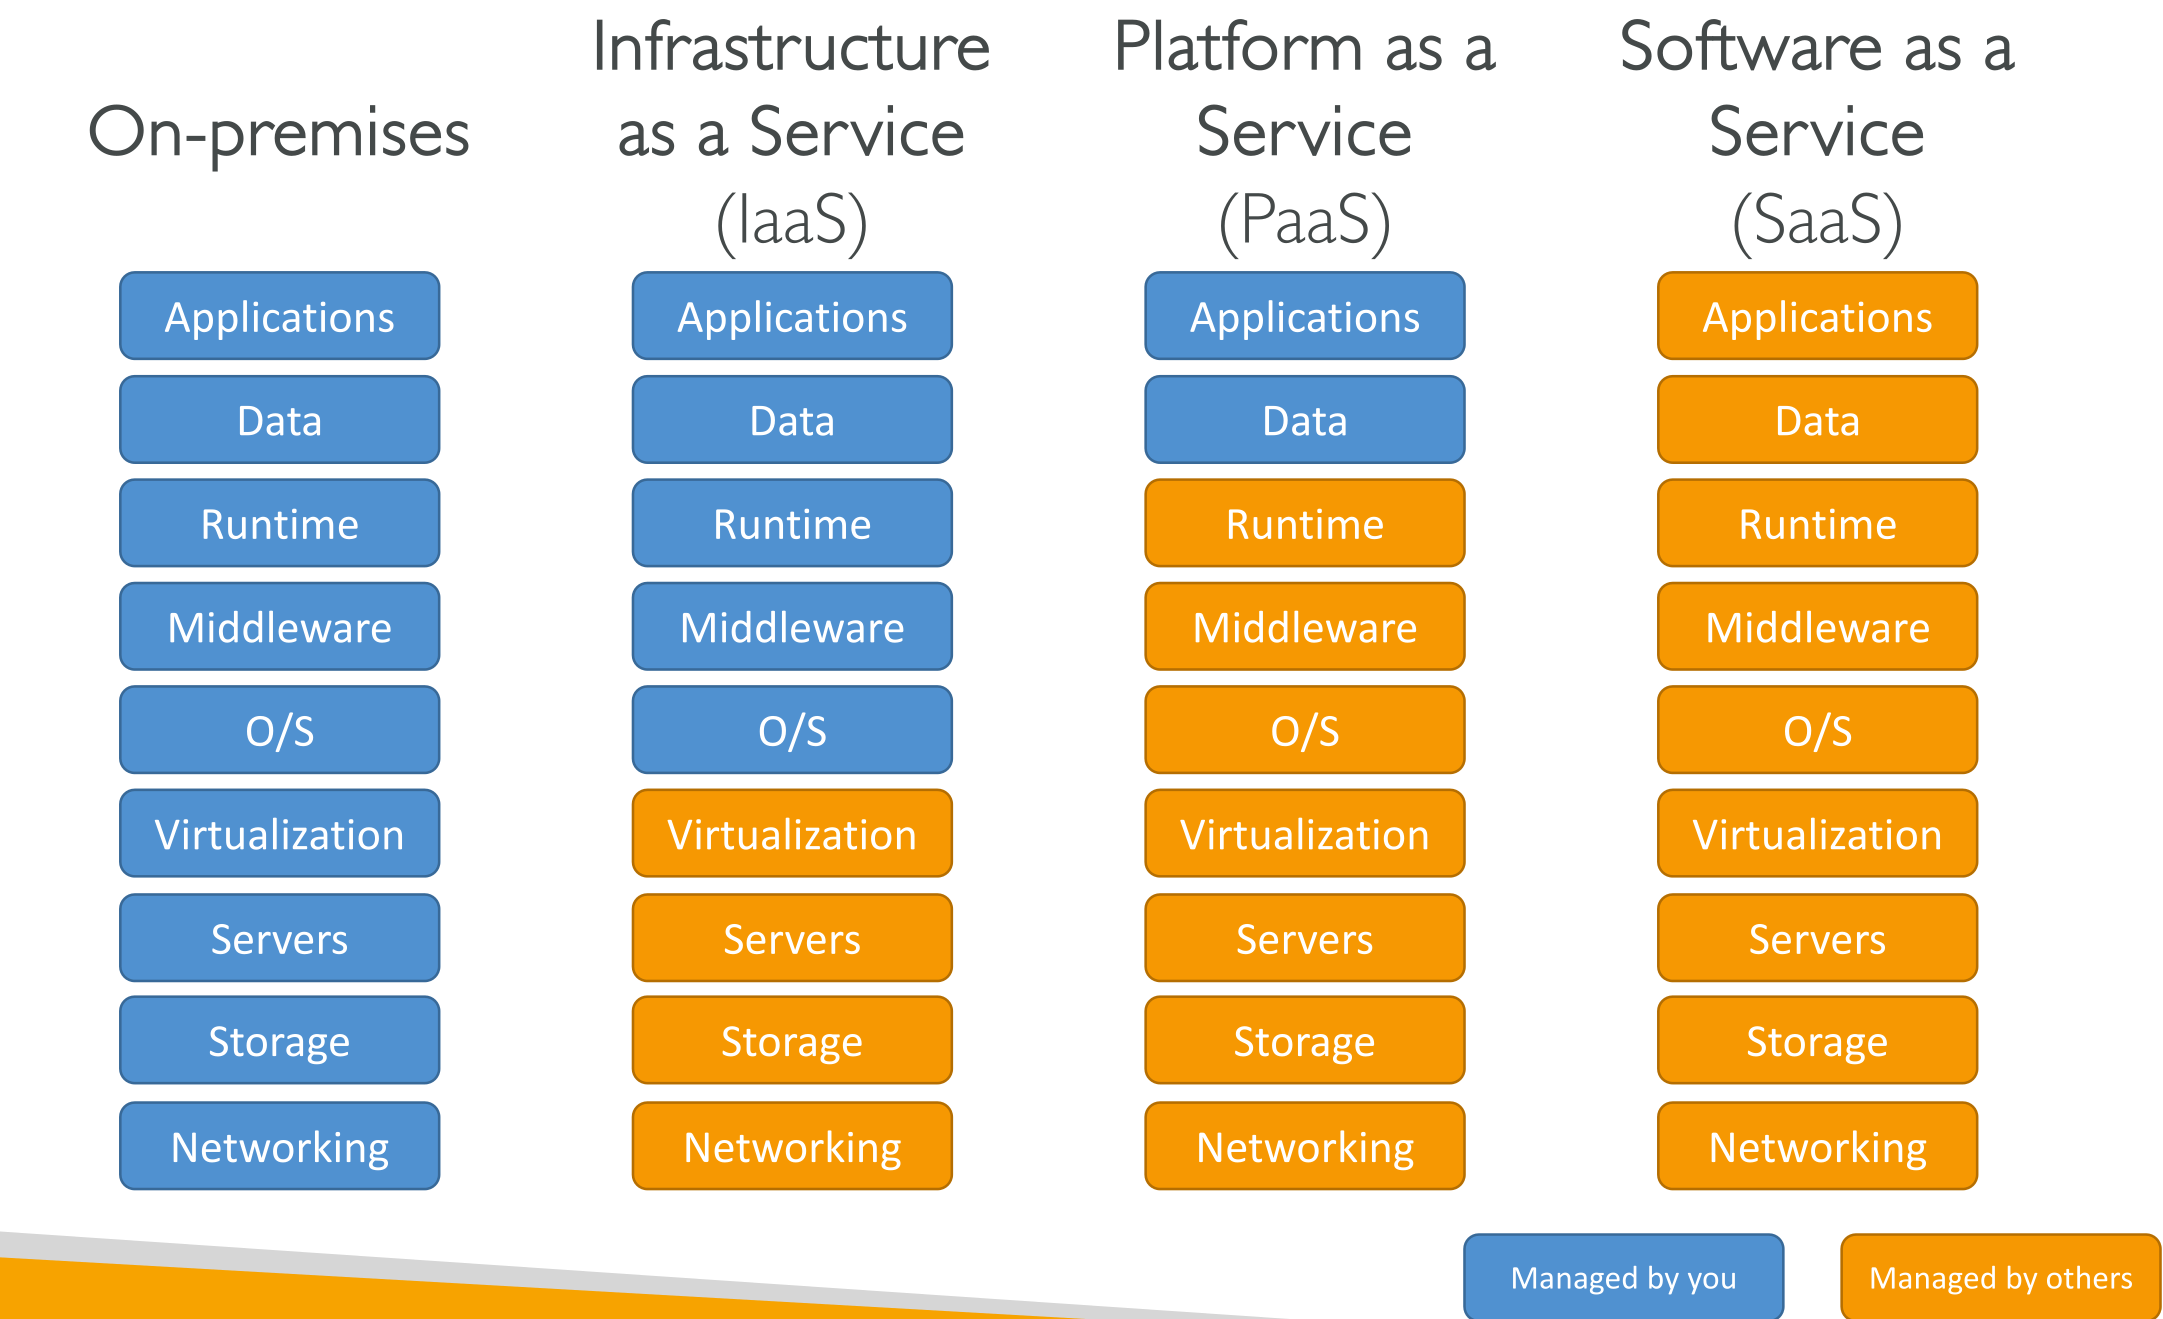
\includegraphics[width=0.4\linewidth]{images/paas-saas-iaas}
	\caption{paas-saas-iaas}
	\label{fig:paas-saas-iaas}
\end{figure}

\subsection[Example of Cloud Computing Types]{Example of Cloud Computing Types \\
	\textit{Ví dụ các loại điện toán đám mây}}
	\begin{itemize}
		\item Infrastructure as a Service
		\begin{itemize}
			\item Amazon EC2 (on AWS)
			\item GCP, Azure, Rackspace, Digital Ocean, Linode
		\end{itemize}
		\item Platform as a Service
		\begin{itemize}
			\item Elastic Beanstalk (on AWS)
			\item Heroku, Google App Engine (GCP), Windows Azure (Microsoft)
		\end{itemize}
		\item Software as a Service
		\begin{itemize}
			\item Many AWS services (ex: Rekognition for Machine Learning)
			\item Google Apps (Gmail), Dropbox, Zoom
		\end{itemize}
	\end{itemize}

\subsection[Pricing of the Cloud - Quick Overview]{Pricing of the Cloud - Quick Overview\\
	\textit{Cách tính phí của Đám mây - Tổng quan nhanh}}

\begin{itemize}
	\item AWS has 3 pricing fundamentals, following the pay-as-you-go pricing model (AWS có 3 nguyên tắc định giá cơ bản, dựa trên mô hình trả tiền theo mức sử dụng)
	\item Compute (Tính toán): Pay for compute time (Trả cho thời gian tính toán)
	\item Storage (Lưu trữ): Pay for data stored in the Cloud (Trả tiền cho lưu trữ dự liệu trên đám mây)
	\item Data transfer OUT of the Cloud: Data transfer IN is free (Truy xuất dữ liệu từ đám mây sẽ bị tính phí: việc tải dữ liệu lên là miễn phí.) 
	\item Solves the expensive issue of traditional IT (Giải quyết bài toán chi phí cao của hạ tầng IT truyền thống)
\end{itemize}

\subsection[AWS Cloud History]{AWS Cloud History\\
	\textit{Lịch sử đám mây AWS}}
	
	\begin{figure}[htbp]
		\centering
		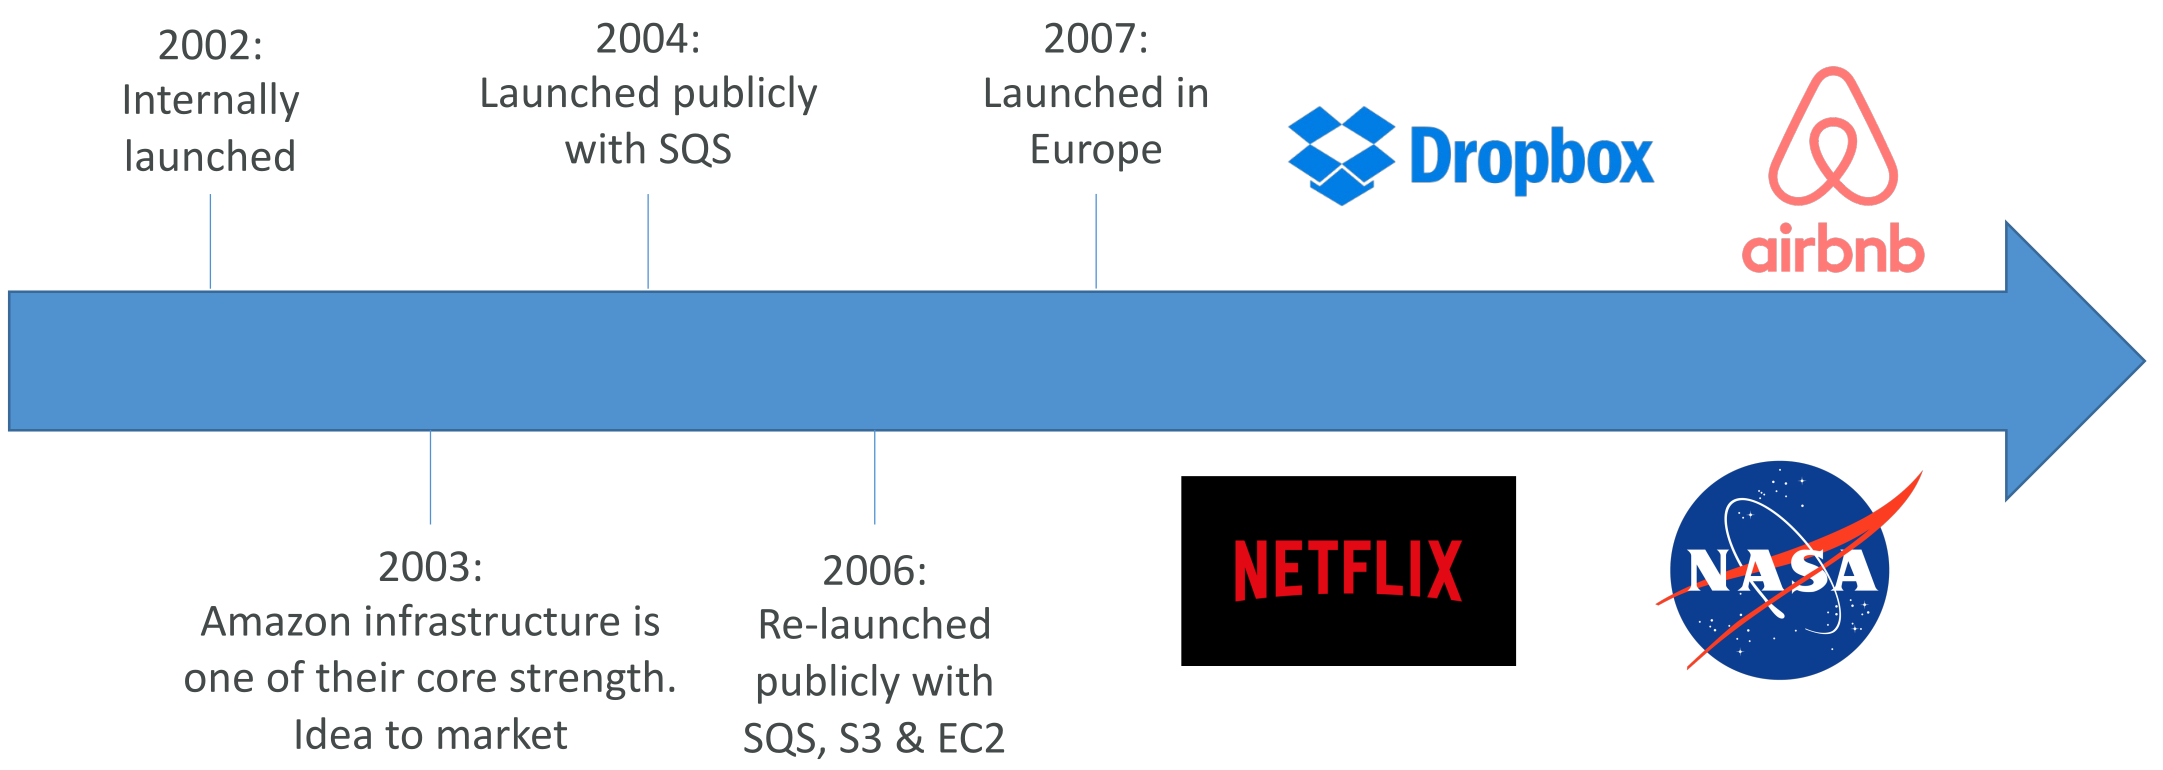
\includegraphics[width=0.8\textwidth]{images/history-aws-cloud}
		\caption{history-aws-cloud}
		\label{fig:history-aws-cloud}
	\end{figure}


\subsection[AWS Cloud Use Cases]{AWS Cloud Use Cases\\
	\textit{Các trường hợp sử dụng đám mây AWS}}
\begin{itemize}
	\item AWS enables you to build sophisticated, scalable applications (AWS cho phép bạn xây dựng các ứng dụng phức tạp và có khả năng mở rộng)
	\item Applicable to a diverse set of industries (Có thể áp dụng cho nhiều ngành công nghiệp khác nhau)
	\item Use cases include
	\begin{itemize}
		\item Enterprise IT, Backup \& Storage, Big data analytics	
		\item Web hosting, Mobile \& Social Apps
		\item Gaming
	\end{itemize}
\end{itemize}

\subsection[AWS Regions]{AWS Regions}

\begin{itemize}
	\item AWS has Regions all around the world (AWS có các Regions  trên khắp thế giới.)
	\item Names can be  us-east-1, eu-west-3, ...(Có thể là us-east-1, eu-west-3)
	\item A region is a cluster of data centers (Một region là một cụm trung tâm dữ liệu.)
	\item Most AWS services are region-scoped (Hầu hết các dịch vụ AWS có phạm vi theo vùng (region).)
\end{itemize}

\subsection[How to choose AWS Region?]{How to choose AWS Region\\
	\textit{Cách chọn một AWS Region?}}
if you need launch a new application, where should you do it?

\begin{itemize}
	\item \textcolor{blue}{\textbf{Compliance}} with data governance and legal requirements: data never leaves a region without your explicit permission (Tuân thủ các yêu cầu về quản trị dữ liệu và pháp lý: dữ liệu không bao giờ rời khỏi khu vực mà không có sự cho phép rõ ràng từ bạn)
	\item \textcolor{blue}{\textbf{Proximity}} to Customer: reduced latency (Gần với khách hàng: giảm độ trễ hệ thống)
	\item \textcolor{blue}{\textbf{Available services}} within a Region: new services and new features aren't available in every Region (Các dịch vụ có sẵn trong khu vực: Các dịch vụ mới và tính năng không có sẵn ở mọi khu vực)
	\item \textcolor{blue}{\textbf{Pricing}}: pricing varies region to region and is transparent in the service pricing page (Giá cả: Giá cả thay đổi từ khu vực này sang khu vực khác và được công khai trên trang giá dịch vụ)
\end{itemize}


\subsection[AWS Availability Zones]{AWS Availability Zones\\
	\textit{AZ}}
	
	\begin{itemize}
		\item Each region has many availability zones (usually 3, min is 3, max is 6). (Example:)
		\begin{itemize}
			\item ap-southeast-2a
			\item ap-southeast-2b
			\item ap-southeast-2c
		\end{itemize}
			\item Each availability zone (AZ) is one or more discrete data centers with redundant power, networking, and connectivity (Mỗi AZ là một hoặc nhiều trung tâm dữ liệu riêng biệt với năng lượng dự phòng, mạng lưới và kết nối dự phòng)
			\item They're separate from each other, so that they're isolated from disasters (Chúng tách rời nhau, nên chúng bị cô lập khỏi thảm họa)
			\item They're connected with hight bandwidth, ultra-low latency networking (AZ được kết nối với băng thông cao, đỗ trễ mạng siêu thấp)
	\end{itemize}
	\begin{figure}[htbp]
		\centering
		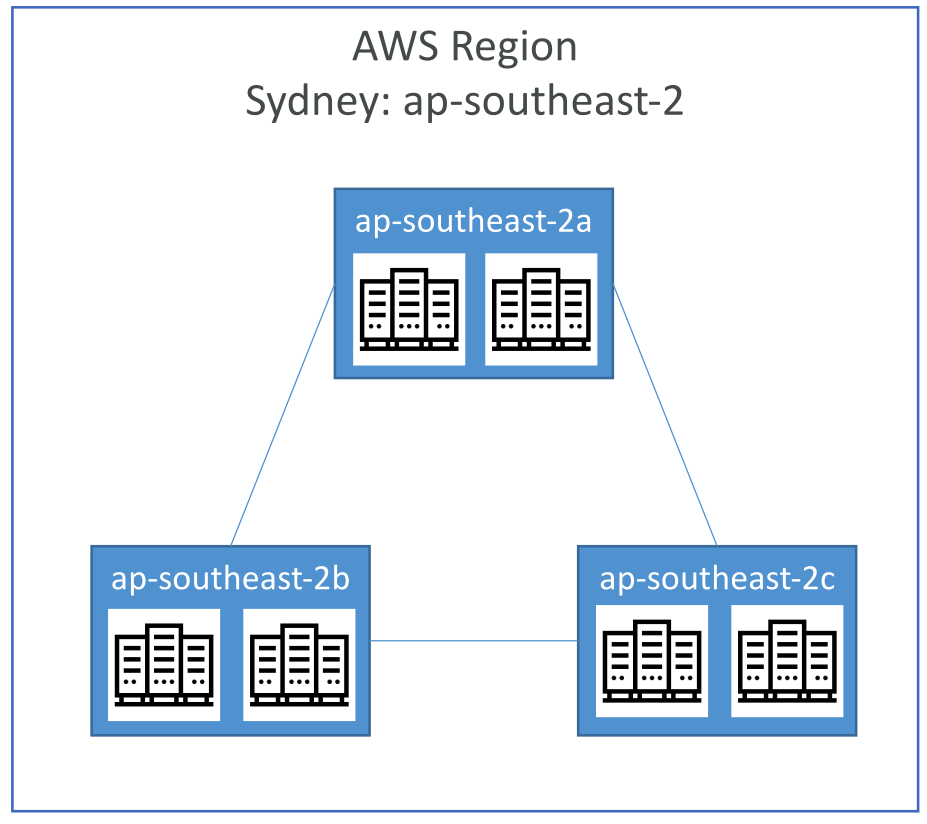
\includegraphics[width=0.8\textwidth]{images/az}
		\caption{Mô hình AZ}
		\label{fig:}
	\end{figure}

\subsection[Shared Responsibility Model Diagram]{Shared Responsibility Model Diagram \\
	\textit{Sơ đồ mô hình chia sẻ trách nhiệm}}

\begin{itemize}
	\item CUSTOMER = RESPONSIBILITY FOR THE SECURITY IN COULD
	\item AWS = RESPONSIBILITY FOR THE SECURITY FOR CLOUD
	\begin{figure}[htbp]
		\centering
		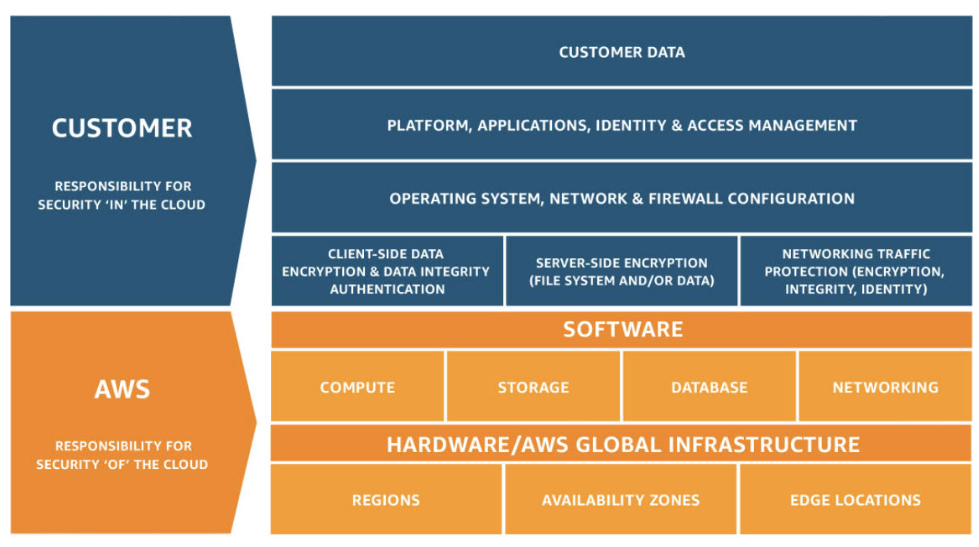
\includegraphics[width=0.8\textwidth]{images/shared-responsibility}
		\caption{shared-responsibility}
		\label{fig:shared-responsibility}
	\end{figure}
\end{itemize}


\subsection[AWS Acceptable Use Policy]{AWS Acceptable Use Policy \\
	\textit{Chính sách sử dụng được chấp nhận của AWS}}

\begin{itemize}
	\item No Illegal, Harmful, or Offensive Use or Content (Bạn không được sử dụng dịch vụ AWS để tạo, truyền, hoặc lưu trữ bất kỳ thứ gì bất hợp pháp, gây hại hoặc mang tính xúc phạm.)
	\item No Security Violations (Không được vi phạm các bảo mật)
	\item No Network Abuse (Không lạm dụng mạng)
	\item No E-mail or Other Message Abuse  (Không lạm dụng email hoặc các hình thức nhắn tin khác)
\end{itemize}

























